\documentclass{standalone}
\usepackage{tikz}
\usetikzlibrary{patterns, positioning}
\usepackage[sfdefault]{ClearSans} %% option 'sfdefault' activates Clear Sans as the default text font
\usepackage[T1]{fontenc}

\begin{document}
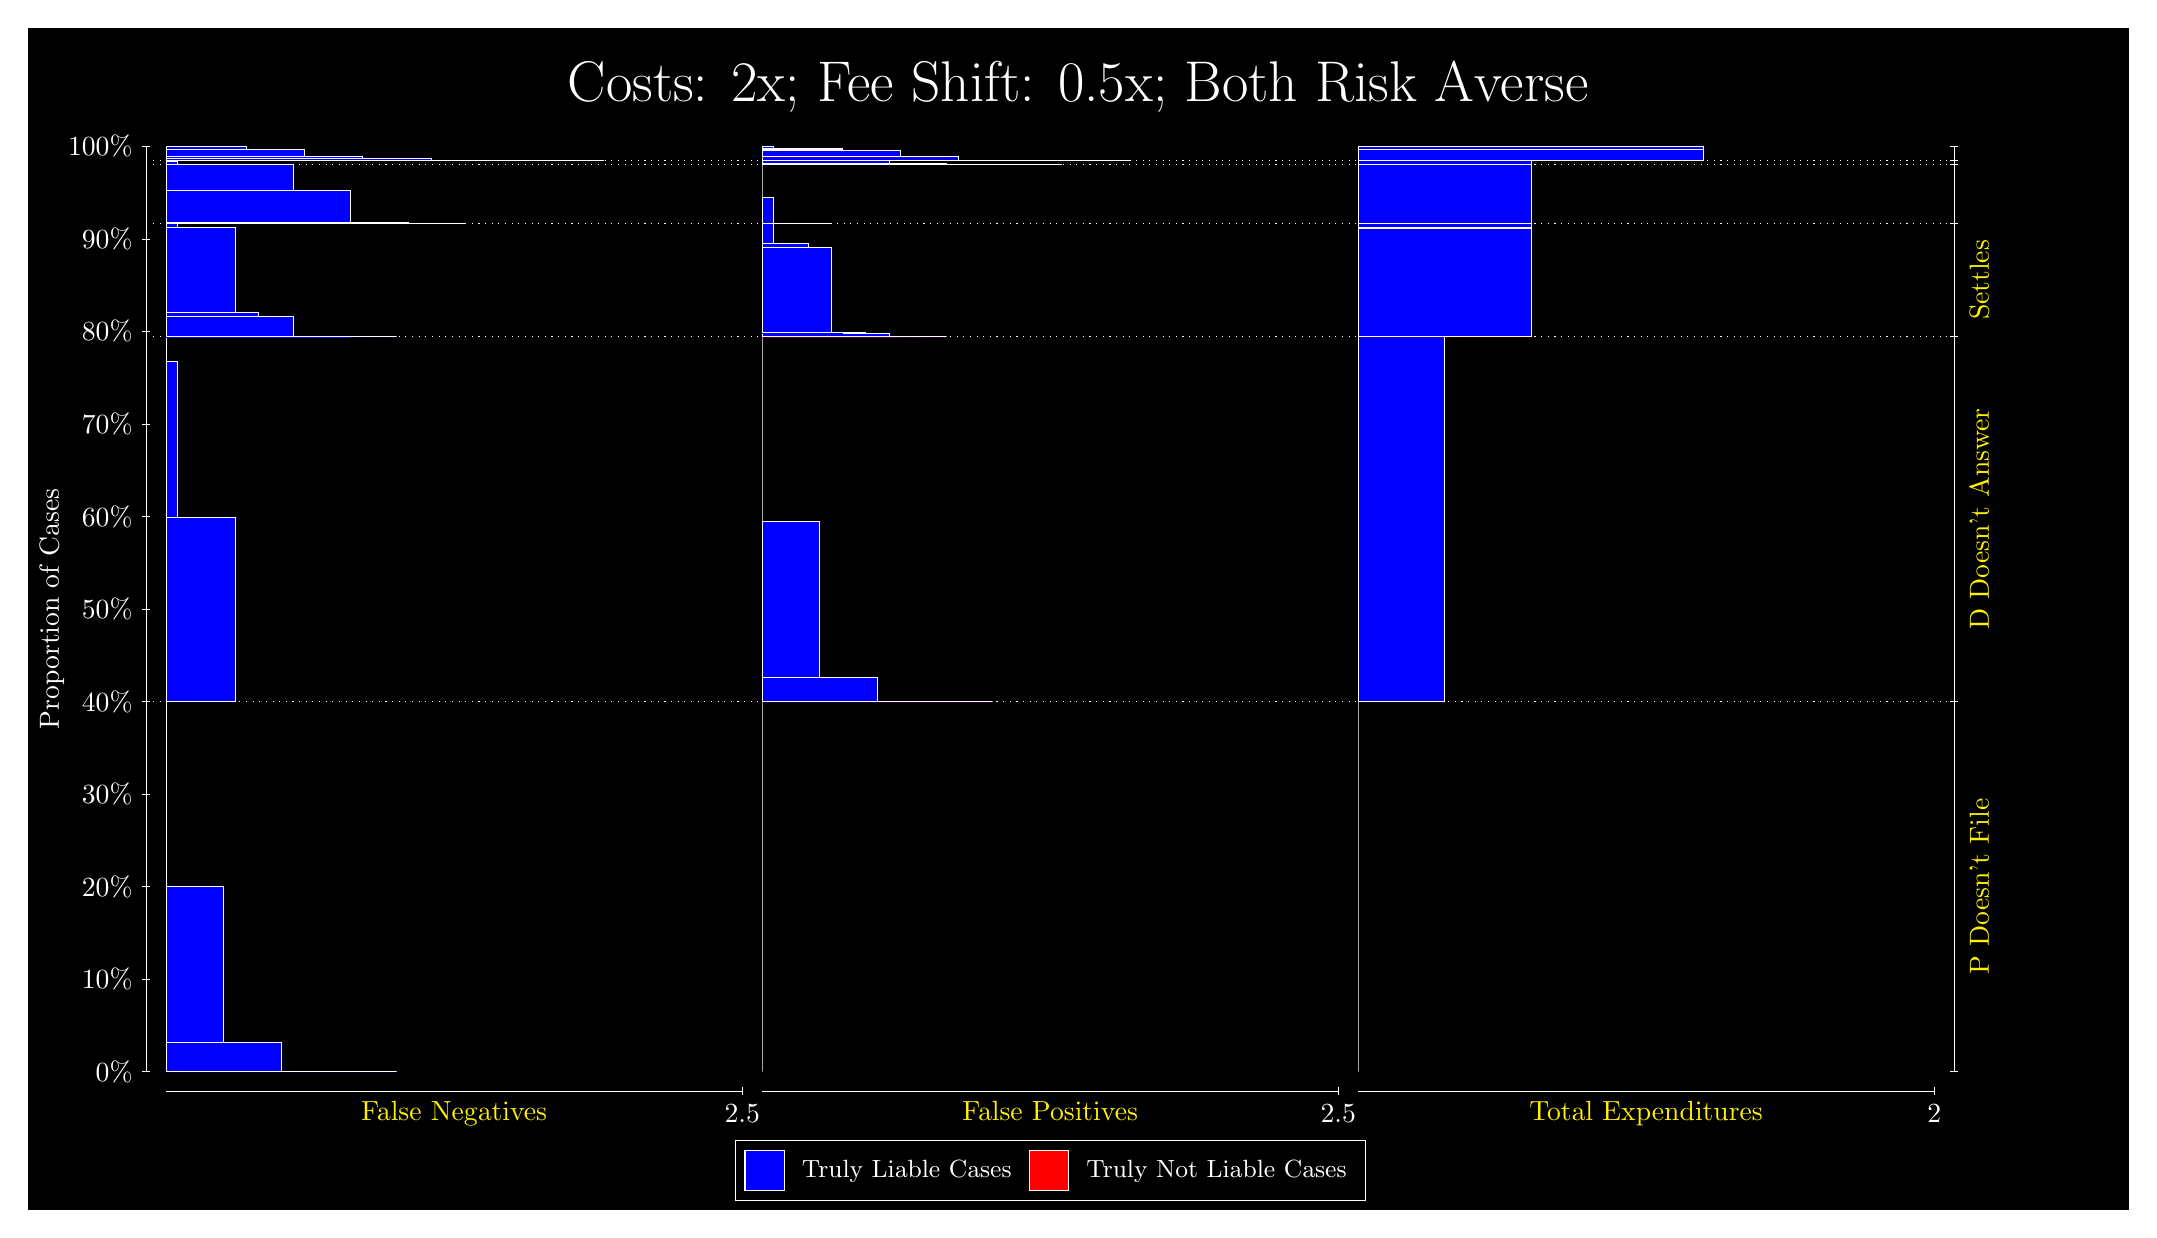
\begin{tikzpicture}
\draw[fill=black] (0,0) rectangle (26.667,15);
\draw[text=white] (0,13.5) rectangle (26.667,15) node[midway] {\huge Costs: 2x; Fee Shift: 0.5x; Both Risk Averse};
\draw[white, very thin] (1.5,1.75) -- (1.5,13.5);
\node[rotate=90, text=white, anchor=center] at (0.3, 7.625) {Proportion of Cases};
\draw[white, very thin] (1.45,1.75) -- (1.55,1.75);
\node[text=white, anchor=east] at (1.45, 1.75) {0\%};
\draw[white, very thin] (1.45,2.925) -- (1.55,2.925);
\node[text=white, anchor=east] at (1.45, 2.925) {10\%};
\draw[white, very thin] (1.45,4.1) -- (1.55,4.1);
\node[text=white, anchor=east] at (1.45, 4.1) {20\%};
\draw[white, very thin] (1.45,5.275) -- (1.55,5.275);
\node[text=white, anchor=east] at (1.45, 5.275) {30\%};
\draw[white, very thin] (1.45,6.45) -- (1.55,6.45);
\node[text=white, anchor=east] at (1.45, 6.45) {40\%};
\draw[white, very thin] (1.45,7.625) -- (1.55,7.625);
\node[text=white, anchor=east] at (1.45, 7.625) {50\%};
\draw[white, very thin] (1.45,8.8) -- (1.55,8.8);
\node[text=white, anchor=east] at (1.45, 8.8) {60\%};
\draw[white, very thin] (1.45,9.975) -- (1.55,9.975);
\node[text=white, anchor=east] at (1.45, 9.975) {70\%};
\draw[white, very thin] (1.45,11.15) -- (1.55,11.15);
\node[text=white, anchor=east] at (1.45, 11.15) {80\%};
\draw[white, very thin] (1.45,12.325) -- (1.55,12.325);
\node[text=white, anchor=east] at (1.45, 12.325) {90\%};
\draw[white, very thin] (1.45,13.5) -- (1.55,13.5);
\node[text=white, anchor=east] at (1.45, 13.5) {100\%};

\draw[white, very thin] (24.457,1.75) -- (24.457,13.5);
\draw[white, very thin] (24.407,1.75) -- (24.507,1.75);
\node[anchor=west] at (24.407, 1.75) {};
\draw[white, very thin] (24.407,6.4489) -- (24.507,6.4489);
\node[anchor=west] at (24.407, 6.4489) {};
\draw[white, very thin] (24.407,11.083) -- (24.507,11.083);
\node[anchor=west] at (24.407, 11.083) {};
\draw[white, very thin] (24.407,12.525) -- (24.507,12.525);
\node[anchor=west] at (24.407, 12.525) {};
\draw[white, very thin] (24.407,13.271) -- (24.507,13.271);
\node[anchor=west] at (24.407, 13.271) {};
\draw[white, very thin] (24.407,13.325) -- (24.507,13.325);
\node[anchor=west] at (24.407, 13.325) {};
\draw[white, very thin] (24.407,13.5) -- (24.507,13.5);
\node[anchor=west] at (24.407, 13.5) {};

\draw[white, very thin, fill=blue] (1.75,1.75) rectangle (4.6775,1.75);
\draw[white, very thin, fill=blue] (1.75,1.75) rectangle (3.9457,1.7532);
\draw[white, very thin, fill=blue] (1.75,1.7532) rectangle (3.2138,2.126);
\draw[white, very thin, fill=blue] (1.75,2.126) rectangle (2.4819,4.1027);
\draw[white, very thin, fill=red] (1.75,4.1027) rectangle (1.75,4.1027);
\draw[white, very thin, fill=blue] (1.75,4.1027) rectangle (1.75,6.4489);
\draw[white, very thin, fill=blue] (1.75,6.4489) rectangle (2.6283,8.7951);
\draw[white, very thin, fill=blue] (1.75,8.7951) rectangle (1.8964,10.769);
\draw[white, very thin, fill=red] (1.75,10.769) rectangle (1.75,10.769);
\draw[white, very thin, fill=blue] (1.75,10.769) rectangle (1.75,11.083);
\draw[white, very thin, fill=blue] (1.75,11.083) rectangle (4.6775,11.083);
\draw[white, very thin, fill=blue] (1.75,11.083) rectangle (4.3848,11.083);
\draw[white, very thin, fill=blue] (1.75,11.083) rectangle (4.092,11.084);
\draw[white, very thin, fill=blue] (1.75,11.084) rectangle (3.9457,11.084);
\draw[white, very thin, fill=blue] (1.75,11.084) rectangle (3.6529,11.087);
\draw[white, very thin, fill=blue] (1.75,11.087) rectangle (3.3602,11.336);
\draw[white, very thin, fill=blue] (1.75,11.336) rectangle (3.2138,11.345);
\draw[white, very thin, fill=blue] (1.75,11.345) rectangle (2.921,11.394);
\draw[white, very thin, fill=blue] (1.75,11.394) rectangle (2.6283,12.475);
\draw[white, very thin, fill=blue] (1.75,12.475) rectangle (2.4819,12.476);
\draw[white, very thin, fill=blue] (1.75,12.476) rectangle (2.1891,12.478);
\draw[white, very thin, fill=blue] (1.75,12.478) rectangle (1.8964,12.525);
\draw[white, very thin, fill=red] (1.75,12.525) rectangle (1.75,12.525);
\draw[white, very thin, fill=blue] (1.75,12.525) rectangle (1.75,12.525);
\draw[white, very thin, fill=blue] (1.75,12.525) rectangle (5.5558,12.525);
\draw[white, very thin, fill=blue] (1.75,12.525) rectangle (4.8239,12.534);
\draw[white, very thin, fill=blue] (1.75,12.534) rectangle (4.092,12.948);
\draw[white, very thin, fill=blue] (1.75,12.948) rectangle (3.3602,13.267);
\draw[white, very thin, fill=blue] (1.75,13.267) rectangle (2.6283,13.271);
\draw[white, very thin, fill=red] (1.75,13.271) rectangle (1.75,13.271);
\draw[white, very thin, fill=blue] (1.75,13.271) rectangle (2.6283,13.273);
\draw[white, very thin, fill=blue] (1.75,13.273) rectangle (1.8964,13.316);
\draw[white, very thin, fill=red] (1.75,13.316) rectangle (1.75,13.316);
\draw[white, very thin, fill=blue] (1.75,13.316) rectangle (1.75,13.325);
\draw[white, very thin, fill=blue] (1.75,13.325) rectangle (7.3123,13.325);
\draw[white, very thin, fill=blue] (1.75,13.325) rectangle (6.5805,13.325);
\draw[white, very thin, fill=blue] (1.75,13.325) rectangle (5.8486,13.329);
\draw[white, very thin, fill=blue] (1.75,13.329) rectangle (5.7022,13.329);
\draw[white, very thin, fill=blue] (1.75,13.329) rectangle (5.1167,13.344);
\draw[white, very thin, fill=blue] (1.75,13.344) rectangle (4.9703,13.344);
\draw[white, very thin, fill=blue] (1.75,13.344) rectangle (4.3848,13.346);
\draw[white, very thin, fill=blue] (1.75,13.346) rectangle (4.2384,13.372);
\draw[white, very thin, fill=blue] (1.75,13.372) rectangle (3.6529,13.372);
\draw[white, very thin, fill=blue] (1.75,13.372) rectangle (3.5065,13.457);
\draw[white, very thin, fill=blue] (1.75,13.457) rectangle (2.921,13.457);
\draw[white, very thin, fill=blue] (1.75,13.457) rectangle (2.7746,13.498);
\draw[white, very thin, fill=blue] (1.75,13.498) rectangle (2.0428,13.5);
\draw[white, very thin, fill=red] (1.75,13.5) rectangle (1.75,13.5);
\draw[white, very thin, fill=blue] (1.75,13.5) rectangle (1.75,13.5);
\draw[white, very thin, fill=red] (9.3189,1.75) rectangle (9.3189,1.75);
\draw[white, very thin, fill=blue] (9.3189,1.75) rectangle (9.3189,6.4489);
\draw[white, very thin, fill=red] (9.3189,6.4489) rectangle (12.246,6.4489);
\draw[white, very thin, fill=blue] (9.3189,6.4489) rectangle (12.246,6.4489);
\draw[white, very thin, fill=blue] (9.3189,6.4489) rectangle (11.515,6.4494);
\draw[white, very thin, fill=blue] (9.3189,6.4494) rectangle (10.783,6.7631);
\draw[white, very thin, fill=blue] (9.3189,6.7631) rectangle (10.051,8.7371);
\draw[white, very thin, fill=blue] (9.3189,8.7371) rectangle (9.3189,11.083);
\draw[white, very thin, fill=red] (9.3189,11.083) rectangle (11.661,11.083);
\draw[white, very thin, fill=blue] (9.3189,11.083) rectangle (11.661,11.083);
\draw[white, very thin, fill=red] (9.3189,11.083) rectangle (11.368,11.083);
\draw[white, very thin, fill=blue] (9.3189,11.083) rectangle (11.368,11.083);
\draw[white, very thin, fill=red] (9.3189,11.083) rectangle (11.075,11.083);
\draw[white, very thin, fill=blue] (9.3189,11.083) rectangle (11.075,11.083);
\draw[white, very thin, fill=blue] (9.3189,11.083) rectangle (10.929,11.13);
\draw[white, very thin, fill=blue] (9.3189,11.13) rectangle (10.636,11.133);
\draw[white, very thin, fill=blue] (9.3189,11.133) rectangle (10.344,11.134);
\draw[white, very thin, fill=blue] (9.3189,11.134) rectangle (10.197,12.215);
\draw[white, very thin, fill=blue] (9.3189,12.215) rectangle (9.9044,12.263);
\draw[white, very thin, fill=blue] (9.3189,12.263) rectangle (9.6116,12.272);
\draw[white, very thin, fill=blue] (9.3189,12.272) rectangle (9.4652,12.522);
\draw[white, very thin, fill=blue] (9.3189,12.522) rectangle (9.3189,12.525);
\draw[white, very thin, fill=red] (9.3189,12.525) rectangle (10.197,12.525);
\draw[white, very thin, fill=blue] (9.3189,12.525) rectangle (10.197,12.529);
\draw[white, very thin, fill=blue] (9.3189,12.529) rectangle (9.4652,12.849);
\draw[white, very thin, fill=blue] (9.3189,12.849) rectangle (9.3189,13.271);
\draw[white, very thin, fill=red] (9.3189,13.271) rectangle (13.125,13.271);
\draw[white, very thin, fill=blue] (9.3189,13.271) rectangle (13.125,13.271);
\draw[white, very thin, fill=blue] (9.3189,13.271) rectangle (12.393,13.271);
\draw[white, very thin, fill=blue] (9.3189,13.271) rectangle (11.661,13.281);
\draw[white, very thin, fill=blue] (9.3189,13.281) rectangle (10.929,13.324);
\draw[white, very thin, fill=blue] (9.3189,13.324) rectangle (10.197,13.325);
\draw[white, very thin, fill=red] (9.3189,13.325) rectangle (14.003,13.325);
\draw[white, very thin, fill=blue] (9.3189,13.325) rectangle (14.003,13.325);
\draw[white, very thin, fill=red] (9.3189,13.325) rectangle (13.271,13.325);
\draw[white, very thin, fill=blue] (9.3189,13.325) rectangle (13.271,13.325);
\draw[white, very thin, fill=red] (9.3189,13.325) rectangle (12.539,13.325);
\draw[white, very thin, fill=blue] (9.3189,13.325) rectangle (12.539,13.328);
\draw[white, very thin, fill=blue] (9.3189,13.328) rectangle (11.807,13.368);
\draw[white, very thin, fill=red] (9.3189,13.368) rectangle (11.807,13.368);
\draw[white, very thin, fill=blue] (9.3189,13.368) rectangle (11.807,13.368);
\draw[white, very thin, fill=red] (9.3189,13.368) rectangle (11.661,13.368);
\draw[white, very thin, fill=blue] (9.3189,13.368) rectangle (11.661,13.368);
\draw[white, very thin, fill=blue] (9.3189,13.368) rectangle (11.075,13.452);
\draw[white, very thin, fill=blue] (9.3189,13.452) rectangle (11.075,13.453);
\draw[white, very thin, fill=red] (9.3189,13.453) rectangle (10.929,13.453);
\draw[white, very thin, fill=blue] (9.3189,13.453) rectangle (10.929,13.453);
\draw[white, very thin, fill=blue] (9.3189,13.453) rectangle (10.344,13.466);
\draw[white, very thin, fill=blue] (9.3189,13.466) rectangle (10.344,13.479);
\draw[white, very thin, fill=blue] (9.3189,13.479) rectangle (10.197,13.481);
\draw[white, very thin, fill=red] (9.3189,13.481) rectangle (10.197,13.481);
\draw[white, very thin, fill=blue] (9.3189,13.481) rectangle (10.197,13.481);
\draw[white, very thin, fill=blue] (9.3189,13.481) rectangle (9.6116,13.481);
\draw[white, very thin, fill=blue] (9.3189,13.481) rectangle (9.6116,13.481);
\draw[white, very thin, fill=blue] (9.3189,13.481) rectangle (9.4652,13.496);
\draw[white, very thin, fill=blue] (9.3189,13.496) rectangle (9.4652,13.496);
\draw[white, very thin, fill=blue] (9.3189,13.496) rectangle (9.3189,13.5);
\draw[white, very thin, fill=red] (16.888,1.75) rectangle (16.888,1.75);
\draw[white, very thin, fill=blue] (16.888,1.75) rectangle (16.888,6.4489);
\draw[white, very thin, fill=red] (16.888,6.4489) rectangle (17.986,6.4489);
\draw[white, very thin, fill=blue] (16.888,6.4489) rectangle (17.986,11.083);
\draw[white, very thin, fill=red] (16.888,11.083) rectangle (19.083,11.083);
\draw[white, very thin, fill=blue] (16.888,11.083) rectangle (19.083,12.462);
\draw[white, very thin, fill=red] (16.888,12.462) rectangle (19.083,12.462);
\draw[white, very thin, fill=blue] (16.888,12.462) rectangle (19.083,12.471);
\draw[white, very thin, fill=red] (16.888,12.471) rectangle (19.083,12.471);
\draw[white, very thin, fill=blue] (16.888,12.471) rectangle (19.083,12.525);
\draw[white, very thin, fill=red] (16.888,12.525) rectangle (19.083,12.525);
\draw[white, very thin, fill=blue] (16.888,12.525) rectangle (19.083,13.271);
\draw[white, very thin, fill=red] (16.888,13.271) rectangle (19.083,13.271);
\draw[white, very thin, fill=blue] (16.888,13.271) rectangle (19.083,13.325);
\draw[white, very thin, fill=red] (16.888,13.325) rectangle (21.279,13.325);
\draw[white, very thin, fill=blue] (16.888,13.325) rectangle (21.279,13.464);
\draw[white, very thin, fill=red] (16.888,13.464) rectangle (21.279,13.464);
\draw[white, very thin, fill=blue] (16.888,13.464) rectangle (21.279,13.5);
\draw[white, dotted] (1.5,6.4489) -- (24.457,6.4489);
\draw[white, dotted] (1.5,11.083) -- (24.457,11.083);
\draw[white, dotted] (1.5,12.525) -- (24.457,12.525);
\draw[white, dotted] (1.5,13.271) -- (24.457,13.271);
\draw[white, dotted] (1.5,13.325) -- (24.457,13.325);
\draw[white, very thin] (1.75,1.5) -- (9.0689,1.5);
\node[text=yellow, anchor=north] at (5.4094, 1.5) {False Negatives};
\draw[white, very thin] (9.0689,1.45) -- (9.0689,1.55);
\node[text=white, anchor=north] at (9.0689, 1.45) {2.5};

\draw[white, very thin] (9.3189,1.5) -- (16.638,1.5);
\node[text=yellow, anchor=north] at (12.978, 1.5) {False Positives};
\draw[white, very thin] (16.638,1.45) -- (16.638,1.55);
\node[text=white, anchor=north] at (16.638, 1.45) {2.5};

\draw[white, very thin] (16.888,1.5) -- (24.207,1.5);
\node[text=yellow, anchor=north] at (20.547, 1.5) {Total Expenditures};
\draw[white, very thin] (24.207,1.45) -- (24.207,1.55);
\node[text=white, anchor=north] at (24.207, 1.45) {2};

\node[text=yellow, centered, rotate=90] at (24.777, 4.0995) {P Doesn't File};
\node[text=yellow, centered, rotate=90] at (24.777, 8.7661) {D Doesn't Answer};
\node[text=yellow, centered, rotate=90] at (24.777, 11.804) {Settles};




\draw (12.978300999999998,1.5) node[draw=none] (baseCoordinate) {};
\begin{scope}[align=center]
        \matrix[scale=0.5, draw=white, below=0.5cm of baseCoordinate, nodes={draw}, column sep=0.1cm]{
            \node[rectangle, draw, minimum width=0.5cm, minimum height=0.5cm, fill=blue] {}; &
            \node[draw=none, font=\small, text=white] (B) {Truly Liable Cases}; &
            \node[rectangle, draw, minimum width=0.5cm, minimum height=0.5cm, fill=red] {}; &
            \node[draw=none, font=\small, text=white] (B) {Truly Not Liable Cases}; \\
            };
\end{scope}

\end{tikzpicture}
\end{document}